\documentclass[ignorenonframetext,t]{beamer}
\usetheme{2ndQuadrantTraining}

\institute[UbuCon LA 2019]{PostgreSQL y yo}
\date{Talca, Chile, agosto 22, 2019}

\setbeamertemplate{caption}[numbered]
\setbeamertemplate{caption label separator}{: }
\setbeamercolor{caption name}{fg=normal text.fg}
%BEGIN 2ndQuadrant
% The following line has been commented since we use the Beamer style
% to set the fonts.
% \usepackage{lmodern}
%END 2ndQuadrant
\usepackage{amssymb,amsmath}
\usepackage{ifxetex,ifluatex}
\usepackage{fancyvrb}
% \usepackage{fixltx2e} % provides \textsubscript
\usepackage{anyfontsize}
\ifnum 0\ifxetex 1\fi\ifluatex 1\fi=0 % if pdftex
  \usepackage[T1]{fontenc}
  \usepackage[utf8]{inputenc}
\else % if luatex or xelatex
  \ifxetex
    \usepackage{mathspec}
  \else
    \usepackage{fontspec}
  \fi
  \defaultfontfeatures{Mapping=tex-text,Scale=MatchLowercase}
  \newcommand{\euro}{€}
\fi
% use upquote if available, for straight quotes in verbatim environments
\IfFileExists{upquote.sty}{\usepackage{upquote}}{}
% use microtype if available
\IfFileExists{microtype.sty}{%
\usepackage{microtype}
\UseMicrotypeSet[protrusion]{basicmath} % disable protrusion for tt fonts
}{}
\usepackage{graphicx,grffile}
\makeatletter
\def\maxwidth{\ifdim\Gin@nat@width>\linewidth\linewidth\else\Gin@nat@width\fi}
\def\maxheight{\ifdim\Gin@nat@height>\textheight0.8\textheight\else\Gin@nat@height\fi}
\makeatother
% Scale images if necessary, so that they will not overflow the page
% margins by default, and it is still possible to overwrite the defaults
% using explicit options in \includegraphics[width, height, ...]{}
\setkeys{Gin}{width=\maxwidth,height=\maxheight,keepaspectratio}

% http://tex.stackexchange.com/questions/3915/image-on-full-slide-in-beamer-package
\usepackage{textpos}
\newcommand<>{\fullsizegraphic}[1]{
  \begin{textblock*}{0cm}(-1cm,-3.2cm)
  \includegraphics[width=\paperwidth]{#1}
  \end{textblock*}
}

% Comment these out if you don't want a slide with just the
% part/section/subsection/subsubsection title:
\AtBeginPart{
  \let\insertpartnumber\relax
  \let\partname\relax
  \frame{\partpage}
}
\AtBeginSection{
  \let\insertsectionnumber\relax
  \let\sectionname\relax
  \frame{\sectionpage}
}
\AtBeginSubsection{
  \let\insertsubsectionnumber\relax
  \let\subsectionname\relax
  \frame{\subsectionpage}
}

\setlength{\emergencystretch}{3em}  % prevent overfull lines
\providecommand{\tightlist}{%
  \setlength{\itemsep}{0.4ex}\setlength{\parskip}{0.6ex}}
\setcounter{secnumdepth}{0}

% :vim:set sw=3:
\newcommand{\linksize}{\scriptsize}
%\newcommand{\textrightarrow}{$\,\to\,$}
\begin{document}

\begin{frame}[plain]
  \titlepage
\end{frame}


\begin{frame}
	\frametitle{Antonín Houska}
  \begin{itemize}
    \item Antonín Houska, \href{mailto:ah@cybertec.at}{ah@cybertec.at}
    \item Postgres contributor since 2012
    \item Working as a Postgres developer for CYBERTEC since 2012
  \end{itemize}
\end{frame}

\begin{frame}
	\frametitle{Álvaro Herrera}
  \begin{itemize}
    \item Álvaro Herrera, \href{mailto:alvherre@kurilemu.de}{alvherre@kurilemu.de}
    \item Postgres contributor since 2002
    \item Working as a Postgres developer for 2ndQuadrant/EDB since 2012
\begin{itemize} \item \linksize Feel free to grab hold of me on hallways to talk about stuff \end{itemize}
  \end{itemize}
\end{frame}

\begin{frame}
  \frametitle{Talk structure}
  \begin{enumerate}
    \item The problem: table bloat
    \item The historical solution: VACUUM FULL
    \item Third-party solutions
	    \begin{itemize}
		    \item \emph{pg\_repack}
		    \item \emph{pg\_squeeze}
	    \end{itemize}
    \item Non-concurrent REPACK
    \item REPACK CONCURRENTLY
  \end{enumerate}
\end{frame}

\section{Historical review}

\begin{frame}
	\frametitle{The problem: table bloat}
\end{frame}

\begin{frame}
	\frametitle{VACUUM FULL}
\end{frame}

\begin{frame}
	\frametitle{\texttt{pg\_repack}}
  \begin{itemize}
    \item Forked from \texttt{pg\_reorg} in 2012 (\texttt{pg\_reorg} started
      in 2008)
    \item SQL and C functions installed on server, but the workflow is
      controlled by a client application
    \item Like VACUUM FULL / CLUSTER it removes the bloat by copying the
      useful data to a new table, swaps the files and drops the new
      table. Exclusive lock is held only during the swap.
    \item Data changes done by applications during the copying are captured by
      triggers and written to a ``log table''. They are applied right before
      the swap.
  \end{itemize}
\end{frame}

\begin{frame}
  \frametitle{\texttt{pg\_repack}}
  \begin{center}
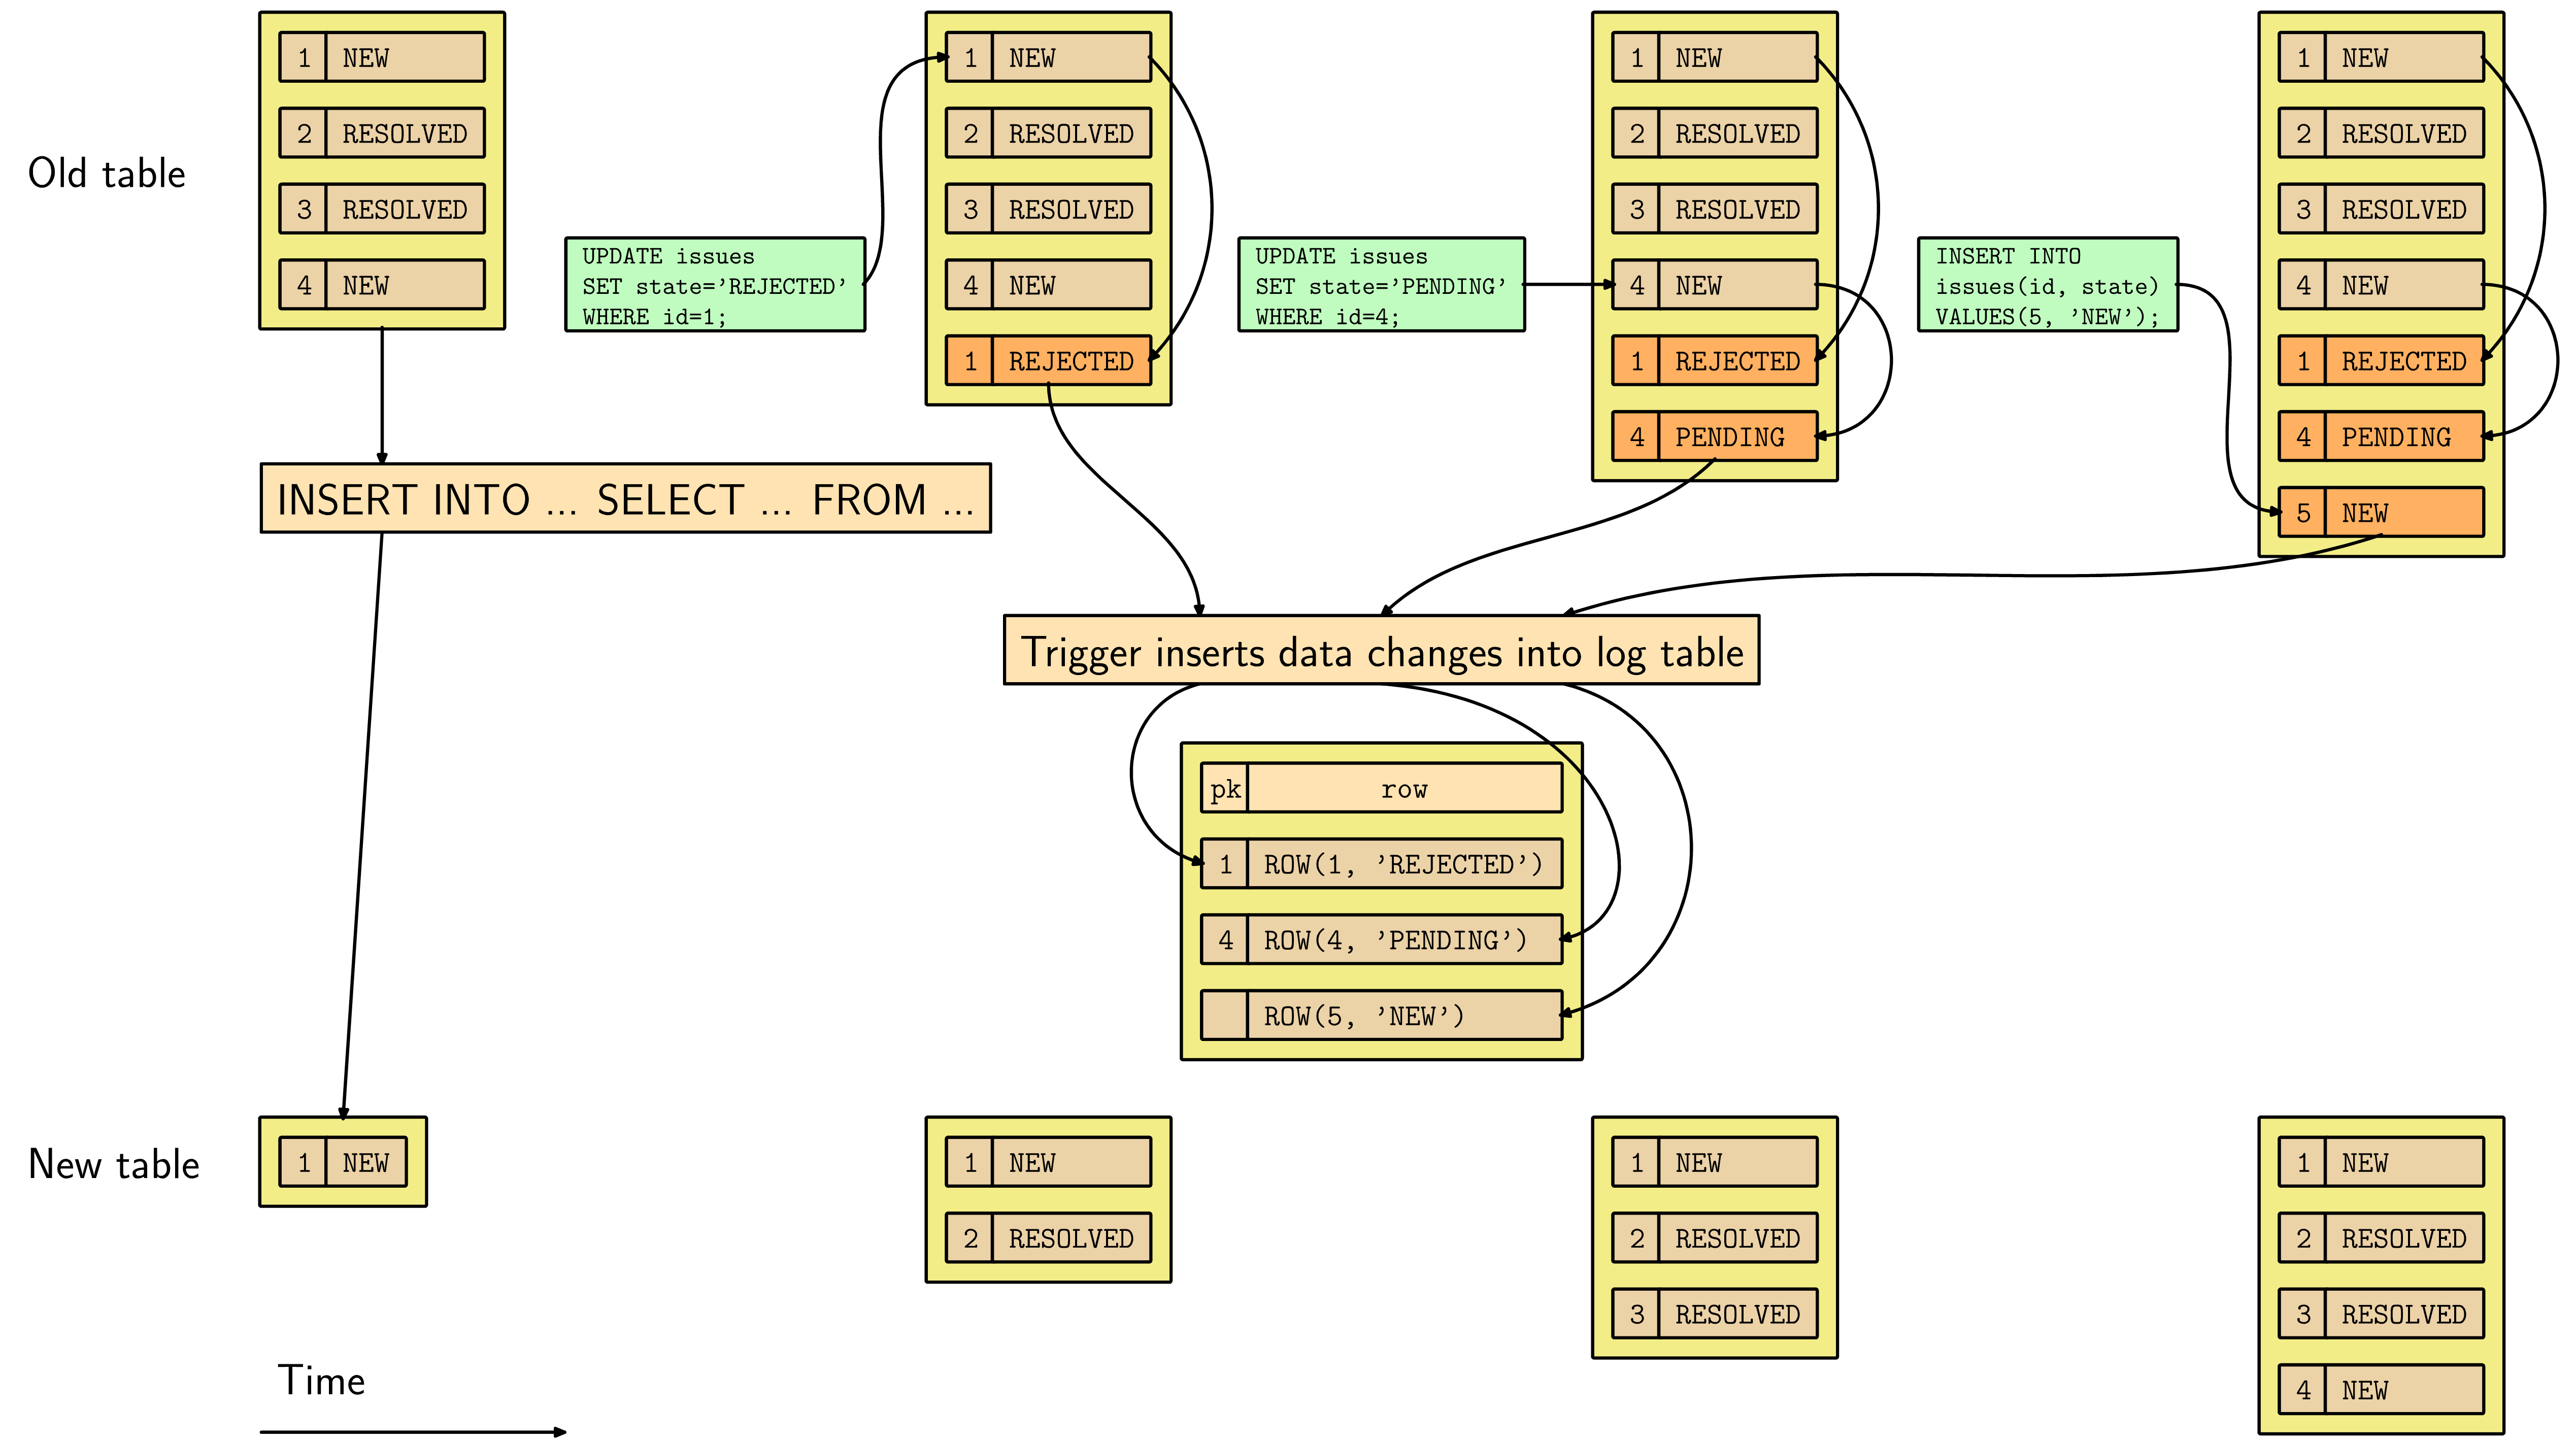
\includegraphics[height=\sizeforimages\textheight]{pg_repack_01.png}
  \end{center}
\end{frame}

\begin{frame}
  \frametitle{\texttt{pg\_repack}}
  \begin{center}
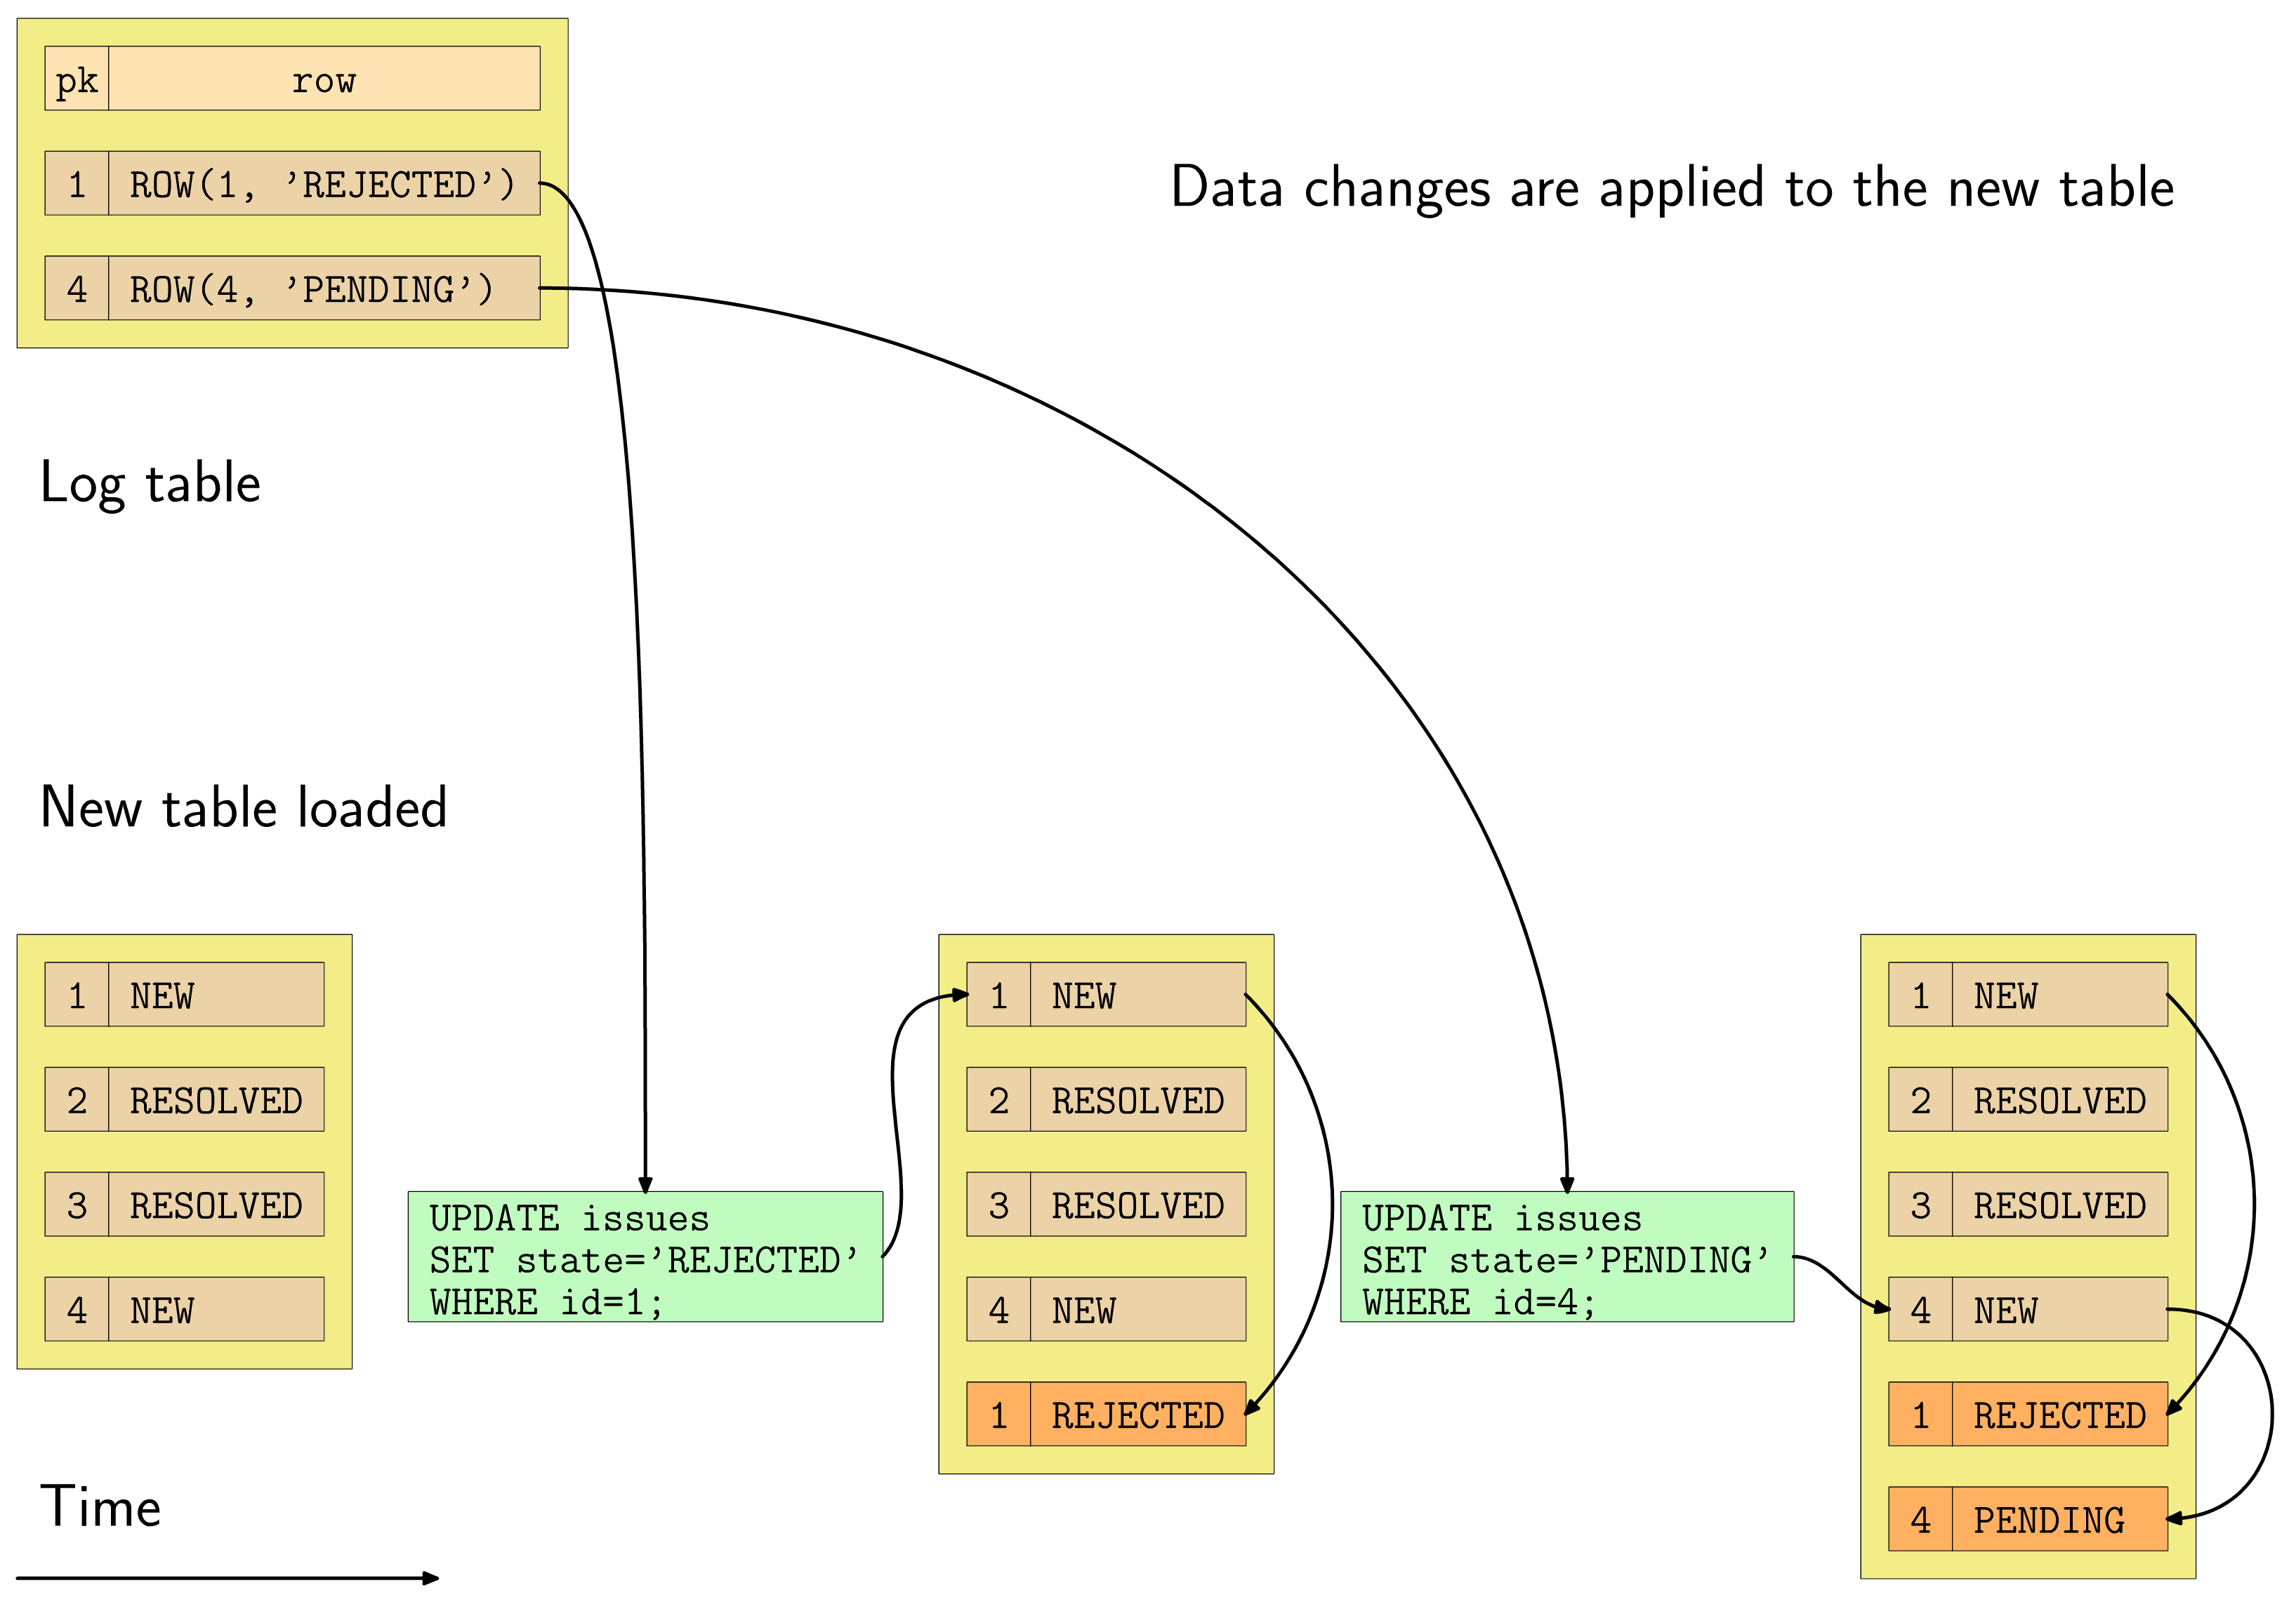
\includegraphics[height=\sizeforimages\textheight]{pg_repack_02.png}
  \end{center}
\end{frame}

\begin{frame}
        \frametitle{\texttt{pg\_squeeze}}
  \begin{itemize}
    \item Started in 2016 (PostgreSQL 9.5)
    \item The idea was to use background worker to launch \texttt{pg\_repack} automatically
    \item \texttt{pg\_repack} is implemented both on server and client side --
      not really suitable for background worker
    \item PostgreSQL 9.4 introduced logical decoding -- I thought it should be
      simpler to use this instead of triggers to capture data changes
    \item Use server API rather than SQL commands to manipulate tables,
      indexes and data.
  \end{itemize}
\end{frame}

\begin{frame}
  \frametitle{\texttt{pg\_squeeze}}
  \begin{center}
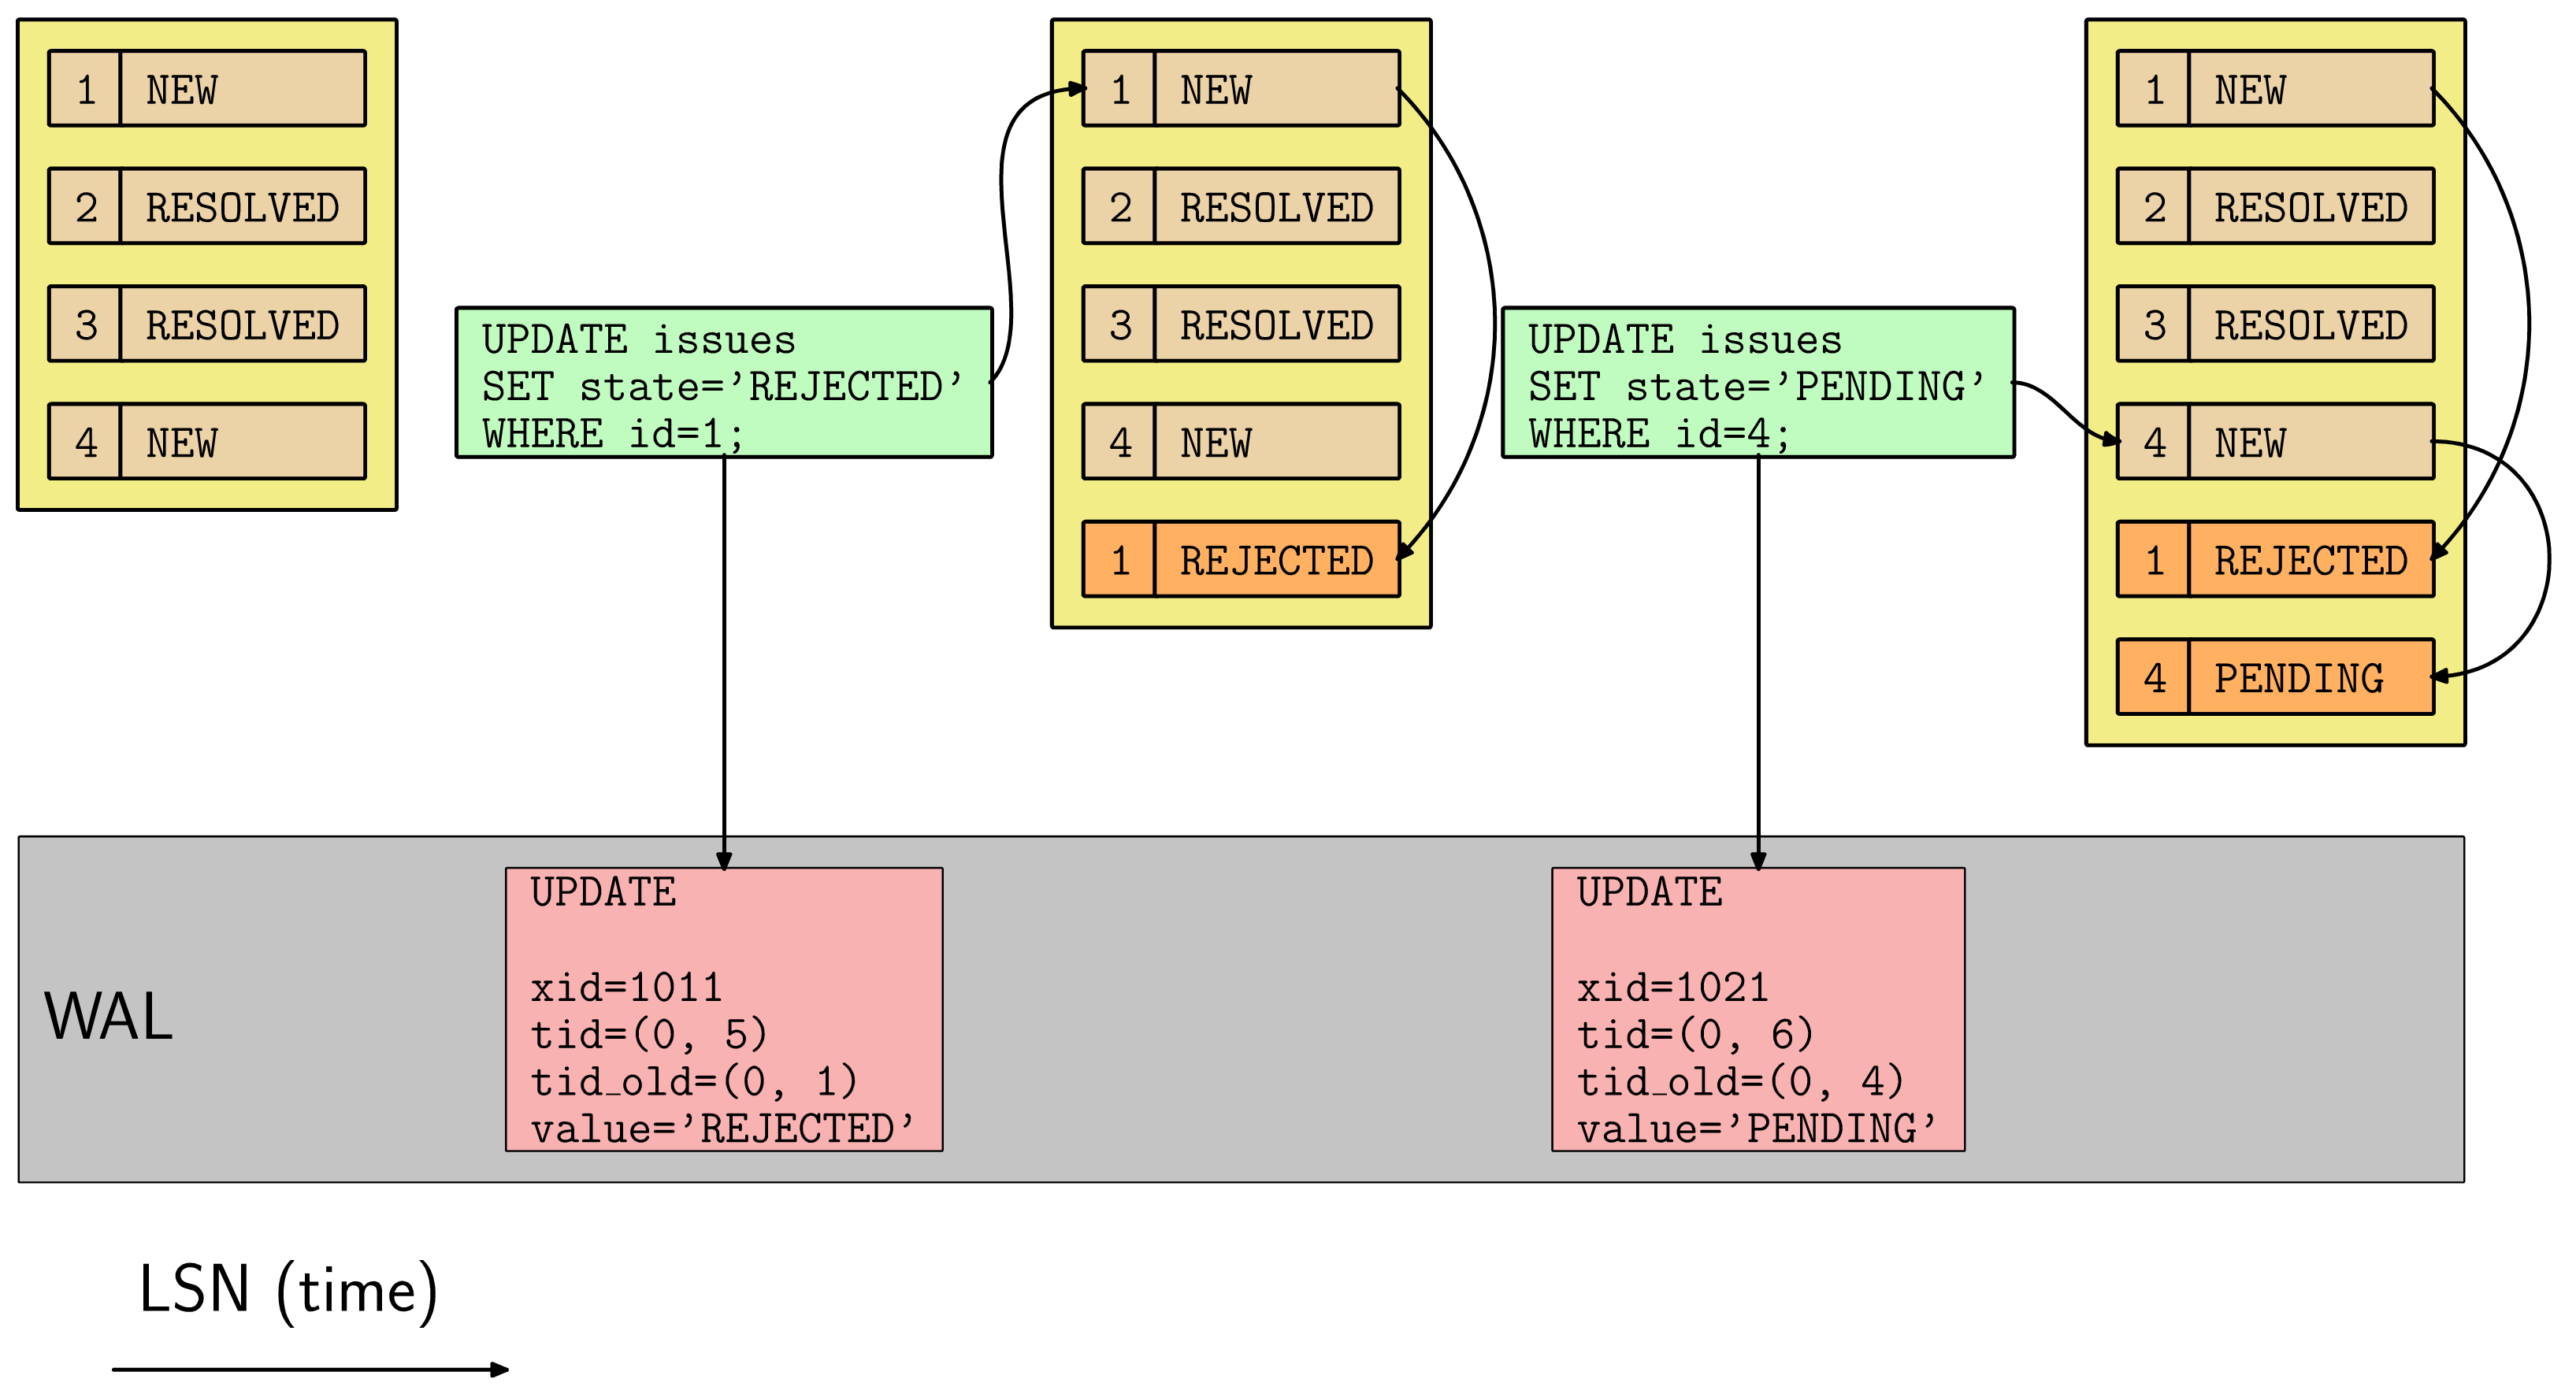
\includegraphics[height=\sizeforimages\textheight]{pg_squeeze_01.png}
  \end{center}
\end{frame}

\begin{frame}
  \frametitle{\texttt{pg\_squeeze}}
  \begin{center}
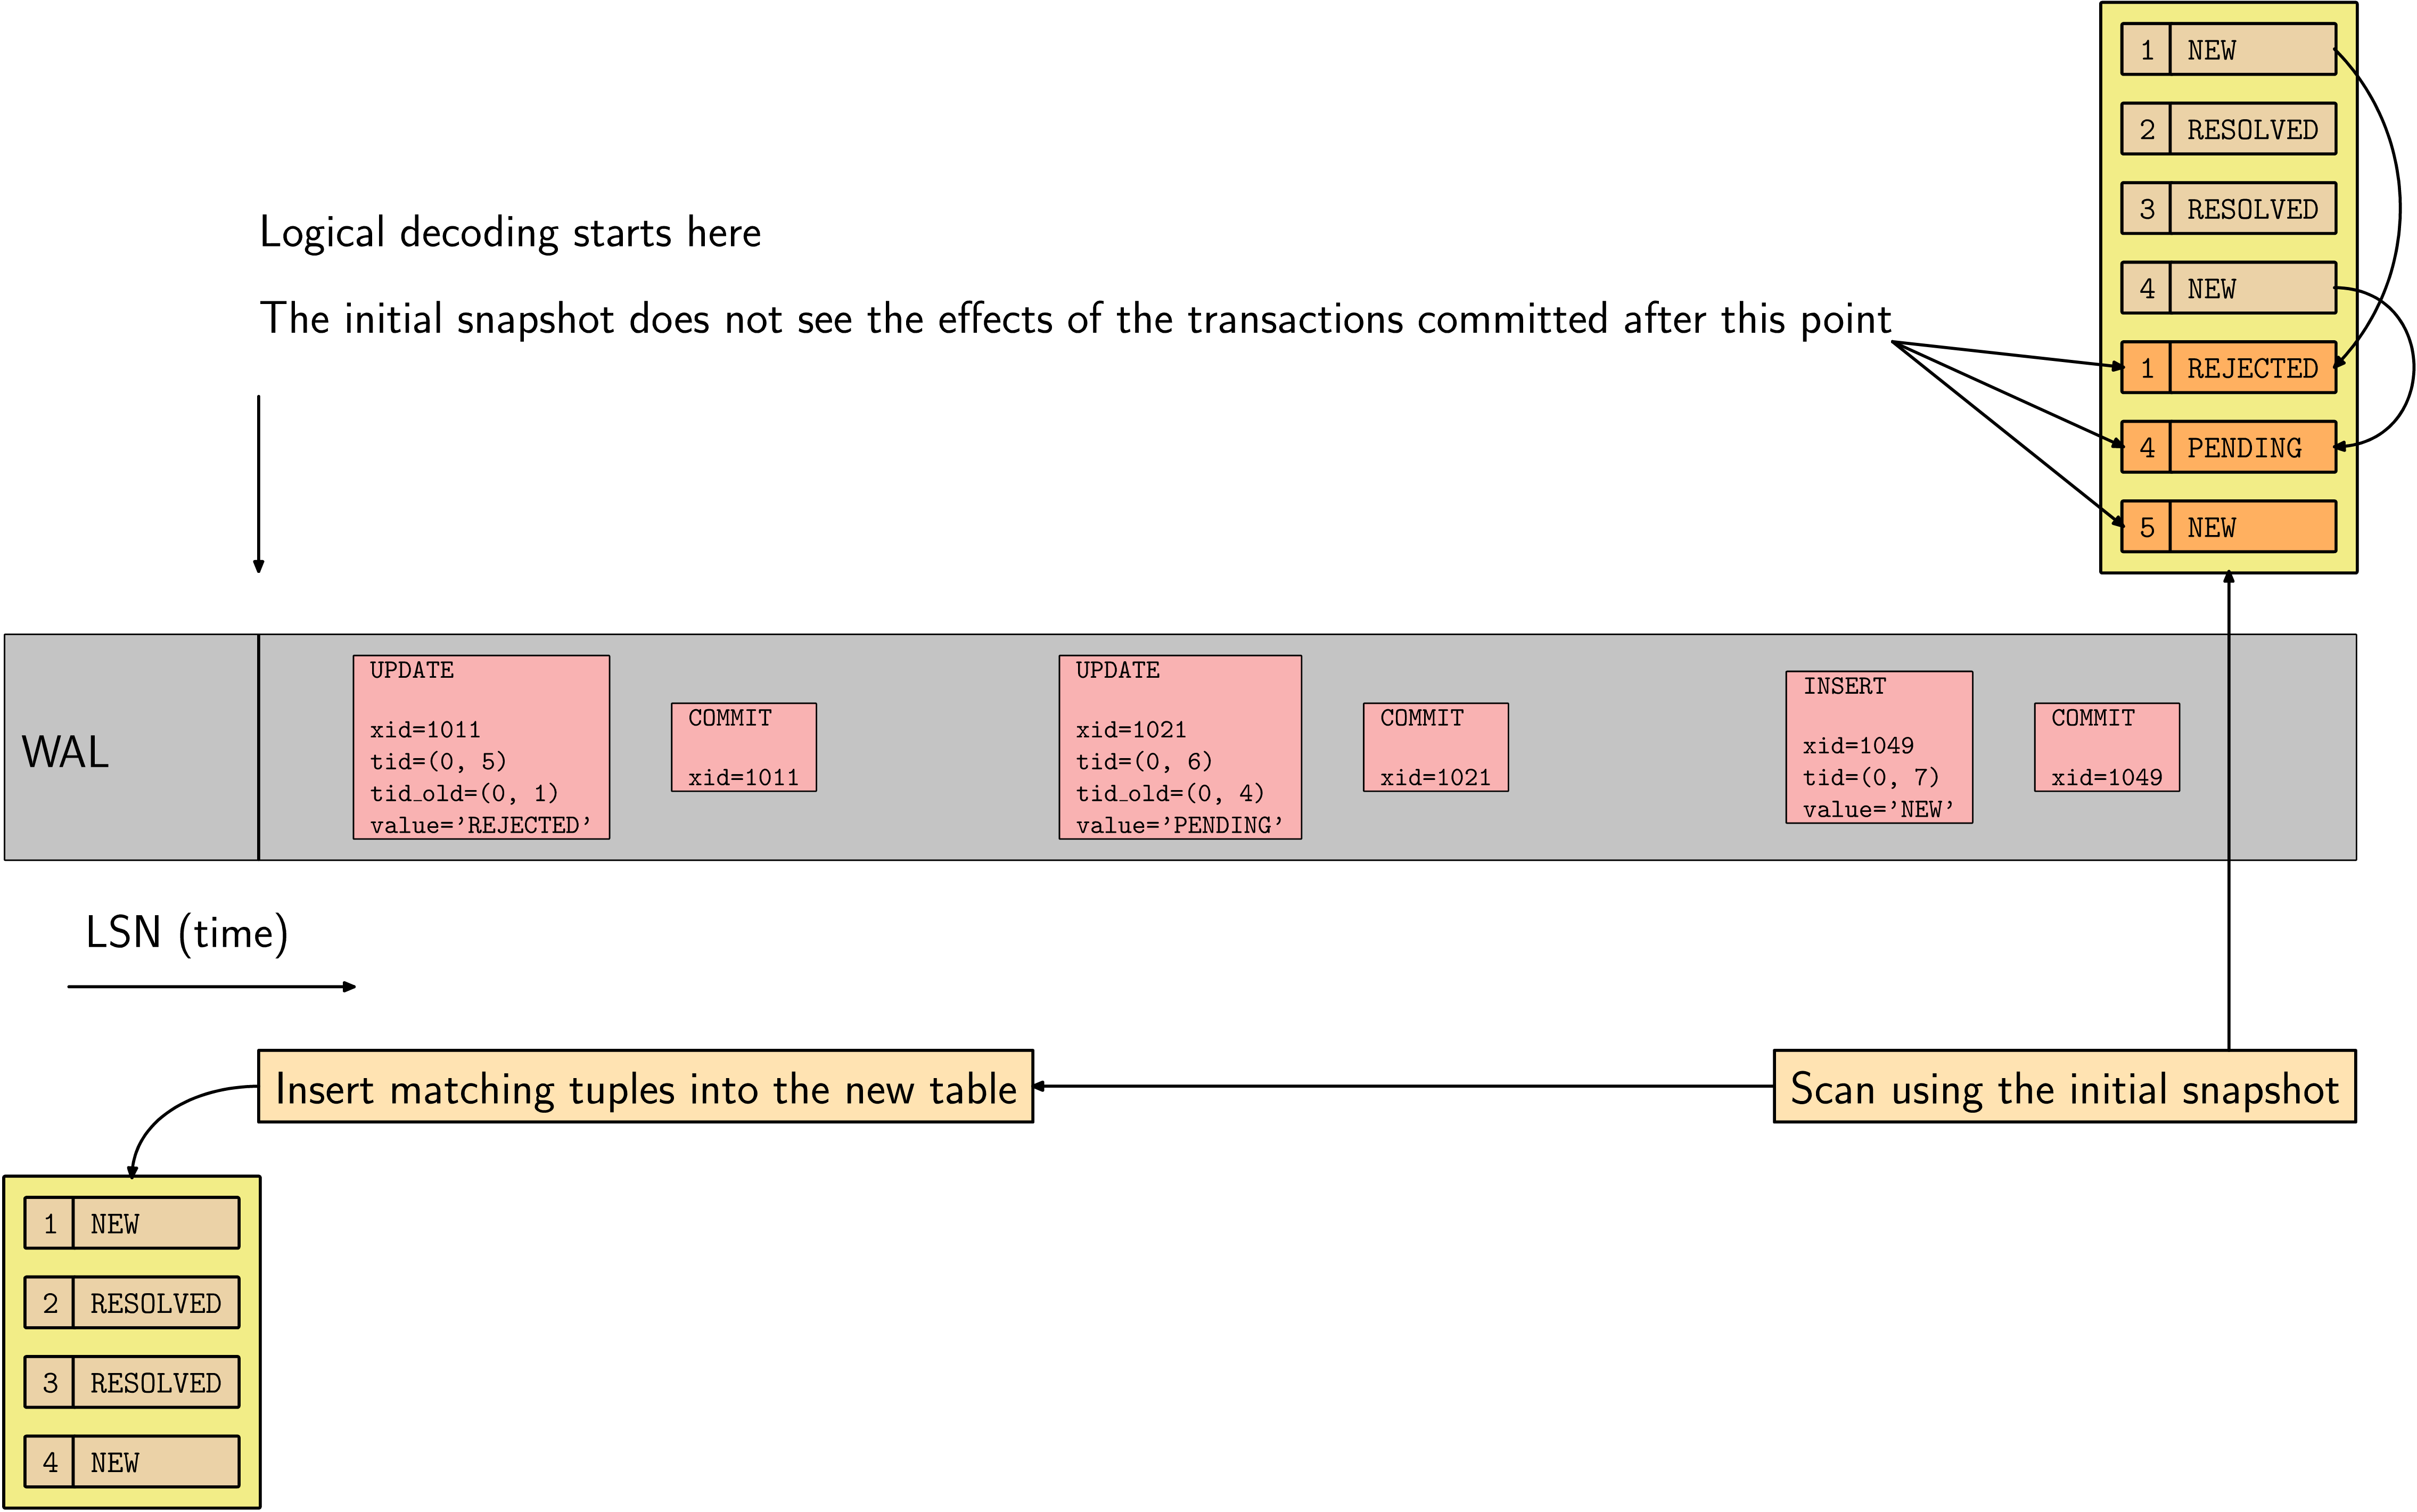
\includegraphics[height=\sizeforimages\textheight]{pg_squeeze_02.png}
  \end{center}
\end{frame}

\begin{frame}
  \frametitle{\texttt{pg\_squeeze}}
  \begin{center}
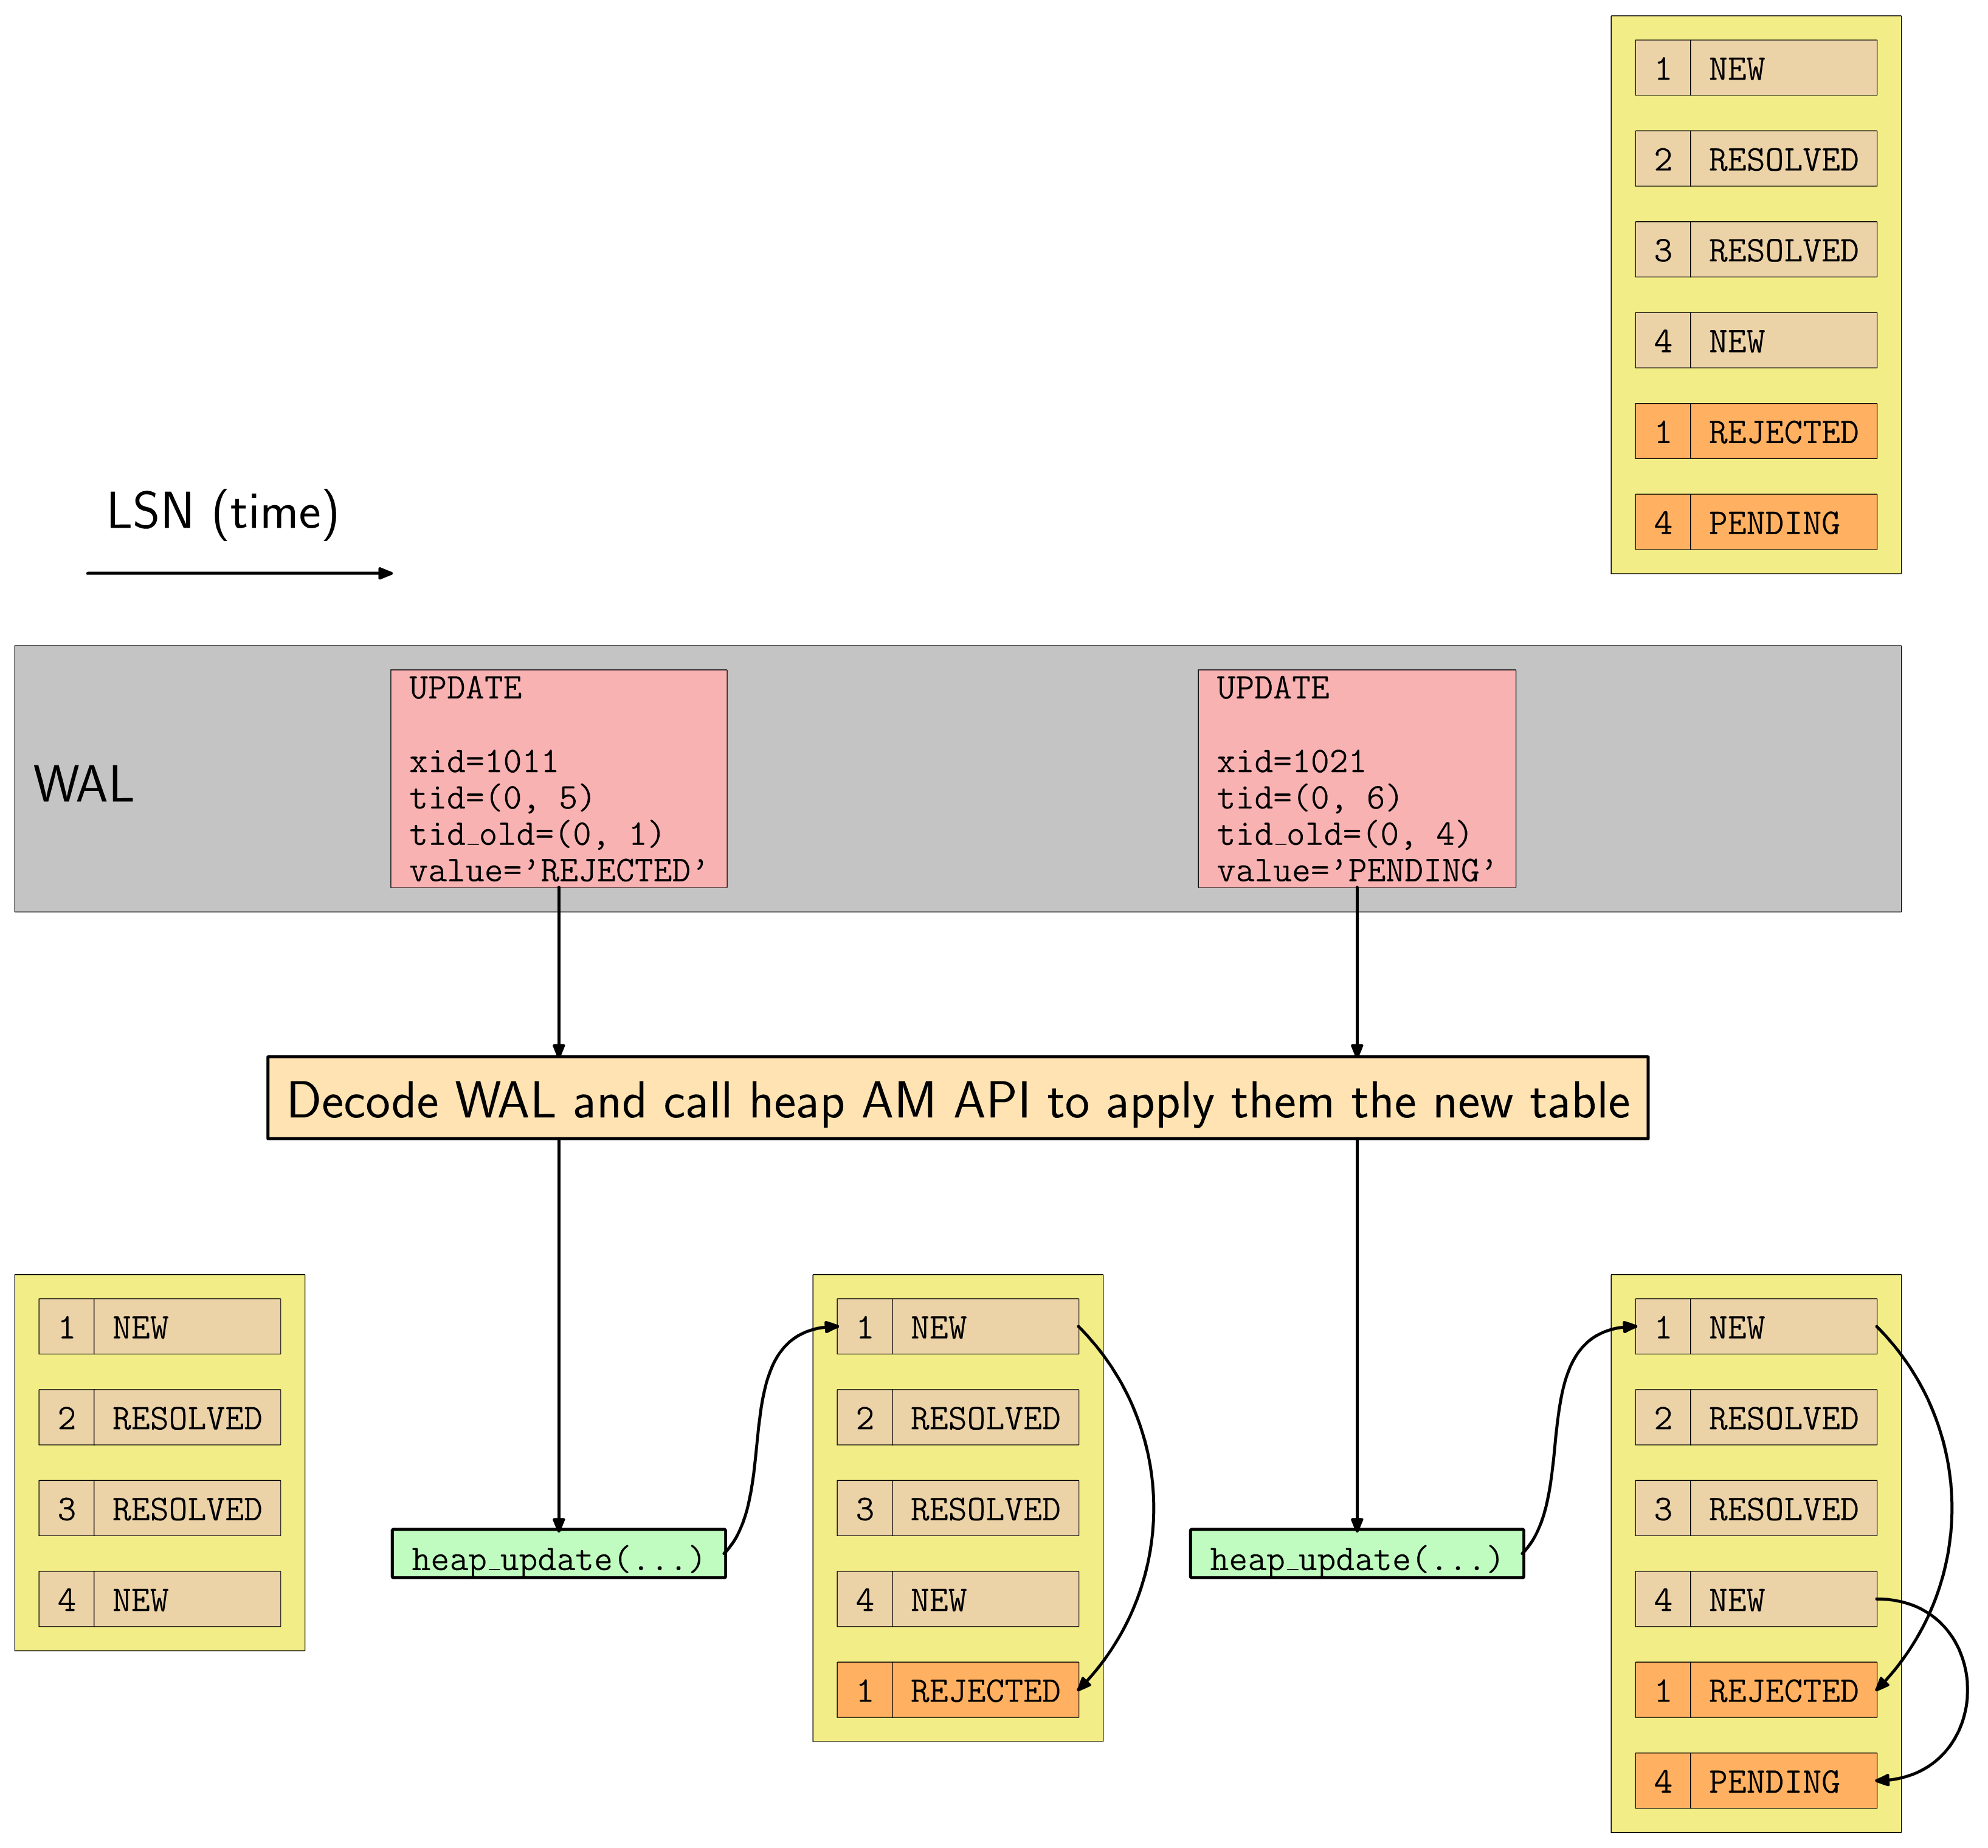
\includegraphics[height=\sizeforimages\textheight]{pg_squeeze_03.png}
  \end{center}
\end{frame}

\begin{frame}
        \frametitle{\texttt{pg\_squeeze}}
%% TODO 1. Disk space requirements, 2. Scheduling, 3. GUC for maximum lock time
%% (probably not used much)
\end{frame}


\section{Repacking done right}
\begin{frame}
	\frametitle{The REPACK command}
\end{frame}

\subsection{Concurrent Repacking}
\begin{frame}
	\frametitle{REPACK CONCURRENTLY}

% TODO (if there's enough time) Explain differences between pg_squeeze and
% REPACK CONCURRENTLY.
%
% 1. pg_squeeze uses AccessShareLock and releases it before it requests
% AccessExclusiveLock (for the file swap), in order to avoid deadlock. If the
% table changed in between, the whole processing is aborted. This approach is
% proably overly cautious. In REPACK CONCURRENTLY, we use
% ShareUpdateExclusiveLock and then simply upgrade it to AccessExclusiveLock,
% so we don't have to check for concurrent catalog changes. (The risk of
% deadlock during the lock upgrade is probably low.)
%
% 2. Since REPACK CONCURRENTLY does not release the ShareUpdateExclusiveLock
% until done, and since this lock conflicts with VACUUM, it does not have to
% care about the xmin horizon (Note: setting the slot's xmin to
% InvalidTransactionId is yet to be implemented.) On the other hand,
% pg_squeeze allows for VACUUM most of the time, so has to block the xmin
% horizon until the initial copy is complete.
%
% 2. Unlike extension, the core code can implement MVCC safety. (Although not
% necessarily in PG 19).
%
% 3. REPACK does not implement scheduling - not sure it's necessary,
% extensions can do that.
\end{frame}


\section{Future work}
\begin{frame}
  \frametitle{Future work}
  %% TODO 1. Logical decoding by background worker, 2. MVCC safety.
\end{frame}


\end{document}
